\documentclass[
% -- opções da classe memoir --
article,			% indica que é um artigo acadêmico
12pt,				% tamanho da fonte
oneside,			% para impressão apenas no recto. Oposto a twoside
a4paper,			% tamanho do papel. 
english,			% idioma adicional para hifenização
brazil,				% o último idioma é o principal do documento
sumario=tradicional
]{abntex2}

% ---
% PACOTES
% ---
\usepackage{lmodern} % Usa a fonte Latin Modern
\usepackage[T1]{fontenc}% Selecao de codigos de fonte.
\usepackage[utf8]{inputenc}% Codificacao do documento (conversão automática dos acentos)
\usepackage{indentfirst}% Indenta o primeiro parágrafo de cada seção.
\usepackage{nomencl} % Lista de simbolos
\usepackage{color}% Controle das cores
\usepackage{graphicx}% Inclusão de gráficos
\usepackage{microtype}% para melhorias de justificação
\usepackage{gensymb}
\usepackage{caption}
\usepackage{booktabs}
\usepackage{footnote}
\usepackage{listings}
\usepackage{longtable}
\usepackage{subcaption}

\definecolor{dkgreen}{rgb}{0,0.6,0}
\definecolor{gray}{rgb}{0.5,0.5,0.5}
\definecolor{mauve}{rgb}{0.58,0,0.82}

\lstset{frame=tb,
  language=C++,
  aboveskip=3mm,
  belowskip=3mm,
  showstringspaces=false,
  columns=flexible,
  basicstyle={\small\ttfamily},
  numbers=left,
  numberstyle=\tiny\color{gray},
  keywordstyle=\color{blue},
  commentstyle=\color{dkgreen},
  stringstyle=\color{mauve},
  breaklines=true,
  breakatwhitespace=true,
  tabsize=4
}

% ---
% Pacotes adicionais, usados apenas no âmbito do Modelo Canônico do abnteX2
% ---
% ---
% Pacotes de citações
% ---
\usepackage[brazilian,hyperpageref]{backref}	 % Paginas com as citações na bibl
%\usepackage[alf,abnt-emphasize=bf]{abntex2cite}	% Citações padrão ABNT
\usepackage[num,overcite,abnt-emphasize=bf]{abntex2cite}	% Citações padrão ABNT
%\citebrackets()
\citebrackets[]
% ---

% ---
% Configurações do pacote backref
% Usado sem a opção hyperpageref de backref
\renewcommand{\backrefpagesname}{Citado na(s) página(s):~}
% Texto padrão antes do número das páginas
\renewcommand{\backref}{}
% Define os textos da citação
\renewcommand*{\backrefalt}[4]{
  \ifcase #1 %
    Nenhuma citação no texto.%
    \or
    Citado na página #2.%
  \else
    Citado nas páginas #2.%
\fi}%
% ---

\graphicspath{{./images/}}

% --- Informações de dados para CAPA e FOLHA DE ROSTO ---
\titulo{IoT: rede LoRa para envio de imagens}
\tituloestrangeiro{IoT: LoRa network for sending images}

\autor{Victor E. Almeida \and Marco A. Guerra}

\local{Foz do Iguaçu}
\data{\today}

\instituicao{%
\par
Universidade do Oeste do Paraná 
\par
UNIOESTE
}
\instituicao{Curso de Ciência da Computação, da Universidade Estadual do Oeste do Paraná (UNIOESTE), Campus Foz do Iguaçu-PR, Brasil}

\preambulo{Escrever Preâmbulo}

\tipotrabalho{Trabalho Acadêmico}
% ---

% ---
% Configurações de aparência do PDF final

% alterando o aspecto da cor azul
\definecolor{blue}{RGB}{41,5,195}

% informações do PDF
\makeatletter
\hypersetup{
  %pagebackref=true,
  pdftitle={\@title}, 
  pdfauthor={\@author},
  pdfsubject={LPWAN},
  pdfcreator={\@author},
  pdfkeywords={LPWAN},
  colorlinks=true,% false: boxed links; true: colored links
  linkcolor=black,% color of internal links
  citecolor=blue,% color of links to bibliography
  filecolor=magenta,% color of file links
  urlcolor=blue,
  bookmarksdepth=4
}
\makeatother
% --- 

% ---
% compila o indice
% ---
\makeindex
% ---

% ---
% Altera as margens padrões
% ---
\setlrmarginsandblock{3cm}{2cm}{*}
\setulmarginsandblock{3cm}{2cm}{*}
\checkandfixthelayout
% ---

% --- 
% Espaçamentos entre linhas e parágrafos 
% --- 

% O tamanho do parágrafo é dado por:
\setlength{\parindent}{1.25cm}
%\setlength{\parindent}{1.5\lineheight}

% Controle do espaçamento entre um parágrafo e outro:
%\setlength{\parskip}{0.2cm}  % tente também \onelineskip
\setlength{\parskip}{\onelineskip}

% Espaçamento simples
\SingleSpacing

% ----
% Início do documento
% ----
\begin{document}
%\pagenumbering{roman}
% Seleciona o idioma do documento (conforme pacotes do babel)
%\selectlanguage{english}
\selectlanguage{brazil}

% Retira espaço extra obsoleto entre as frases.
\frenchspacing 

% ----------------------------------------------------------
% ELEMENTOS PRÉ-TEXTUAIS
% ----------------------------------------------------------

%---
%
% Se desejar escrever o artigo em duas colunas, descomente a linha abaixo
% e a linha com o texto ``FIM DE ARTIGO EM DUAS COLUNAS''.
%\twocolumn[    		% INICIO DE ARTIGO EM DUAS COLUNAS
%
%---

% página de titulo principal (obrigatório)
%\imprimircapa
%\begin{center}
\maketitle
%{\centered\maketitle\imprimirlocal\imprimirinstituicao}
%\imprimirtitulo
%\vspace{.5cm}

%\imprimirinstituicao
%\end{center}

% titulo em outro idioma (opcional)

% resumo em português
\begin{resumoumacoluna}
    Redes utilizando comunicação via LoRa possibilitaram que dispositivos troquem mensagens a longas distâncias e gastando pouca energia. Tendo em vista as limitações de transferência de dados dessas redes este trabalho implementa uma rede para envio de imagens utilizando algoritmos e técnicas já consolidadas de redes de computadores para enviar as imagens em diversas partes e garantir sua integridade. Para implementação dessa rede foram utilizados dispositivos como esp32 e esp32-cam que executam o algoritmo de stop and wait. Uma vez implementada a rede pode-se observar que o tempo médio de envio de uma mensagem LoRa é de 2 segundos, sendo assim podendo enviar imagens de 6810 bytes em 1 minuto.

    % De 100 a 250 palavras
    % frases curtas
    % tem que falar de:
        % objetivo
        % matérias e métodos
        % resultados
        % concluir
  \textbf{Palavras-chave}: LoRa, Rede LPWAN, envio de imagens.
  \vspace{\onelineskip}
  \noindent
\end{resumoumacoluna}

% resumo em inglês
\renewcommand{\resumoname}{Abstract}
\begin{resumoumacoluna}
  \begin{otherlanguage*}{english}
      Networks using communication via LoRa made it possible for devices to exchange messages over long distances and using little energy. Observing the data transfer limitations of these networks, this work implements a network for sending images using algorithms and techniques already consolidated in computer networks to send images in several parts and guarantee their integrity. Devices such as esp32 and esp32-cam were used to implement this network, which execute the stop and wait algorithm. Once the network is implemented, it can be observed that the average time for sending a LoRa message is 2 seconds, thus being able to send images of 6810 bytes in 1 minute.
    \vspace{\onelineskip}
    \noindent

    \textbf{Keywords}: LoRa, LPWAN Network, sending images.
  \end{otherlanguage*}  
\end{resumoumacoluna}

%\listoffigures

%\listoftables

\cleardoublepage

%] % FIM DE ARTIGO EM DUAS COLUNAS
% ---

% ----------------------------------------------------------
% ELEMENTOS TEXTUAIS
% ----------------------------------------------------------

\textual

% ----------------------------------------------------------
% Introdução
% ----------------------------------------------------------
\section{Introdução}\label{Introdução}
Redes LoRa e LoRaWAN possibilitaram a comunicação de dispositivos com baixo consumo energético a longas distâncias\cite{bor2016lora}, porém a largura de banda utilizada e a taxa de transmissão ainda são limitadas, sendo assim o presente trabalho propõe a implementação de uma rede LoRa para envio de imagens.

Para atender esse objetivo, primeiramente na seção~\ref{Definições} buscou compreender conceitos tais como o que são~\nameref{Redes LPWAN} seção~\ref{Redes LPWAN}, o que é~\nameref{LoRa} seção~\ref{LoRa}, e por fim o que é~\nameref{IoT} seção~\ref{IoT}.

Uma vez visto os conceitos, na seção~\ref{Materiais e métodos} expõe-se os \nameref{Dispositivos} utilizados seção~\ref{Dispositivos}, e os principais algoritmos e protocolos na seção~\ref{Protocolos}. Em seguida apresenta-se uma~\nameref{Proposta de Arquitetura}, e em seguida sua implementação na seção~\ref{Implementação}. Por fim é apresentado os resultados obtidos e conclusões nas seções~\ref{Resultados} e~\ref{Conclusão} respectivamente.

\section{Definições}\label{Definições}
\subsection{Redes LPWAN}\label{Redes LPWAN}
LPWAN, \textit{Low Power Wide Area Network}, são redes que alcançam longas distâncias gastando pouca energia, normalmente utilizadas para enviar poucos dados\cite{introducao_lpwan_2017}. Dentre as tecnologias mais utilizadas estão SigFox e LoRa. 
\begin{figure}[!htb]
    \centering
    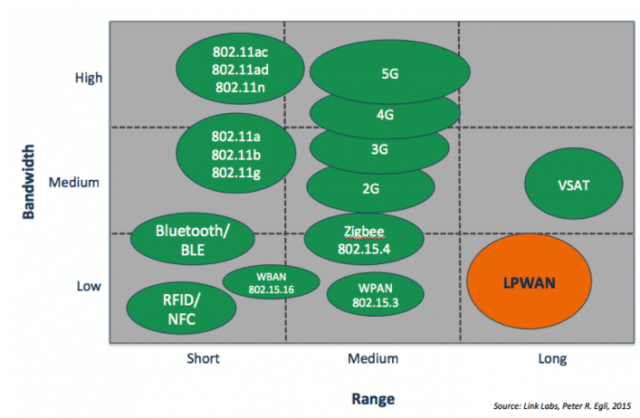
\includegraphics[width=.9\textwidth]{Comparativo-algumas-redes}
    \caption{\label{fig:Comparativo-algumas-redes}Comparando Largura de Banda e distância das redes\cite{introducao_lpwan_2017}}
\end{figure}

\subsection{LoRa}\label{LoRa}
LoRa, \textit{Long Range}, é uma tecnologia que atua na camada física do modelo OSI para o envio e recebimento de dados. Criado e mantido de forma proprietária pela empresa Semtech\cite{bor2016lora} o mesmo utiliza comunicação através de ondas na frequência de radio, para codificar o envio de dados focando em abarcar longas distância a um baixo custo energético. Nesse sentido, uma rede LoRa é formada por diversas antenas\cite{siteLorawan}, que se comunicam utilizando a tecnologia de \textit{Chirp Spread Spectrum}\cite{davcev2018iot} uma tecnologia de comunicação militar adaptada para uso comercial de baixo custo\cite{siteLorawan} tais antenas possuem alcance de até 15 km em áreas rurais\cite{adelantado2017understanding}, bem como uma taxa média de duração de bateria de 10 anos\cite{adelantado2017understanding}.

\subsection{IoT}\label{IoT}
O termo \textit{Internet of Things (IOT)}, em português internet das coisas foi elaborado pelo britânico, Kevin Ashton, em 1999\cite{tzounis2017internet} e se refere de forma geral a uma rede que conecta diversas ``coisas'' a internet, através de software, com o objetivo de trocar informações\cite{defIot}, tais ``coisas'' podem ser sensores, microcontroladores ou até mesmo objetos que nunca imaginamos tais como geladeiras, televisores, entre outros.

A estrutura do \textit{internet of things} é baseada em três camadas principais\cite{tzounis2017internet}:
\begin{itemize}
	\item \textbf{Camada de percepção}: É uma camada que envolve sensores, hardware e obtém-se dados relevantes a respeito dos fenômenos meteorológicos, biológicos ou físicos tais como  temperatura e umidade do solo\cite{kizito2008frequency}, do ar\cite{mesas2015open}, índice de área foliar\cite{bauer2016potential}, quantidade de gás SO$_{2}$\cite{karimi2018web}, PH do solo\cite{karimi2018web} entre muitos outros.
	\item \textbf{Camada de comunicação}: Responsável por enviar os dados coletados pela camada de percepção supracitada para outras camadas, quer sejam aplicações que vão analisar tais dados ou para grandes bancos de dados ou até mesmo para serviços na nuvem.
	\item \textbf{Camada de aplicação}: camada a qual trás sentido aos dados coletados pelos sensores, pois é nesse momento que ocorre o processamento dos dados e a apresentação dos mesmos. Nos trabalhos lidos durante a produção desta revisão bibliográfica, essa camada será responsável principalmente por mostrar ao agricultor informações relevantes de forma simples e compreensível, bem como informá-lo qual o melhor momento para plantar\cite{kath2019soil}, ou em quais lugares da plantação tem doenças\cite{trilles2019development}.
\end{itemize}

\cleardoublepage
\section{Materiais e métodos}\label{Materiais e métodos}
\subsection{Dispositivos}\label{Dispositivos}

\begin{figure}[h!]
  \centering
  \begin{subfigure}[b]{0.3\linewidth}
    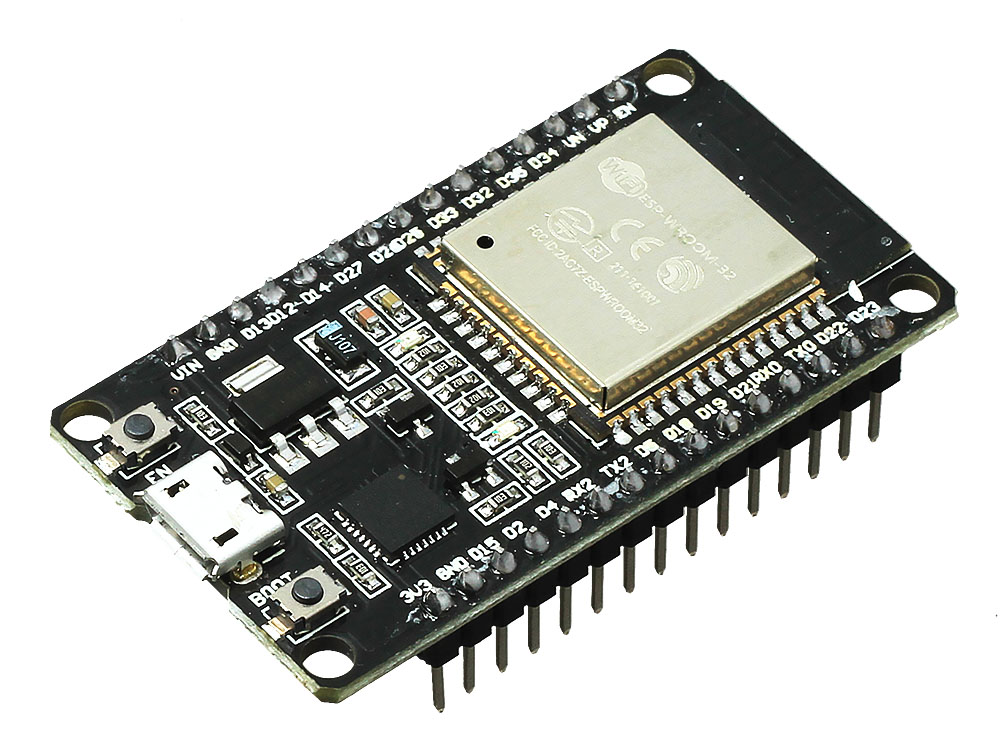
\includegraphics[width=\linewidth]{esp}
    \caption{ESP32}
  \end{subfigure}
  \begin{subfigure}[b]{0.3\linewidth}
    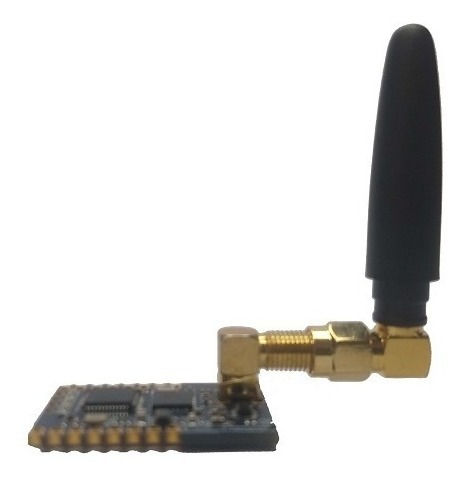
\includegraphics[width=\linewidth]{lora}
    \caption{LoRaMESH EndDivice}
  \end{subfigure}
  \begin{subfigure}[b]{0.3\linewidth}
    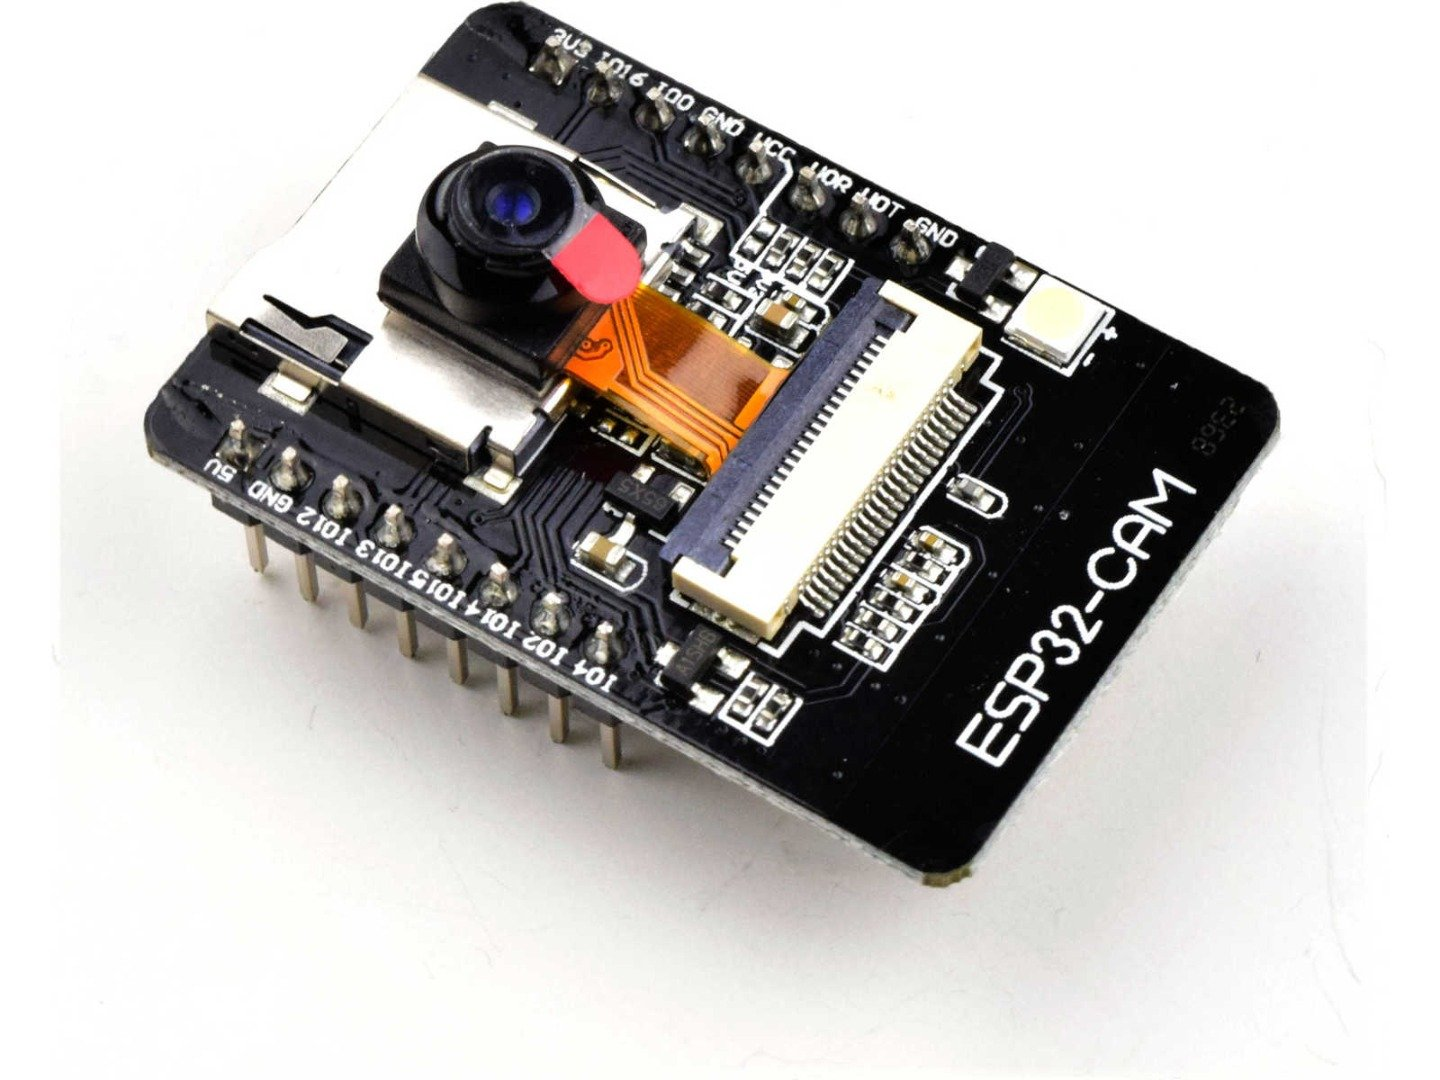
\includegraphics[width=\linewidth]{espcam}
    \caption{ESP32-CAM}
  \end{subfigure}
  \caption{Dispositivos utilizados na aplicação}
  \label{fig:coffee}
\end{figure}

\subsubsection{LoRaMESH EndDivice}\label{LoRaMESH EndDivice}
Para acessar a tecnologia de camada física LoRa utilizou o Módulo LoRaMESH homologado pela ANATEL\cite{lora_radioenge}, o qual possui diversos parâmetros variáveis tais como: \textit{Spreading Factor}, \textit{Coding rate}, Largura de banda de até 500 kHz.

A configuração e utilização do dispositivo é feita através de duas interfaces de comunicação serial (UART), sendo a primeira utilizada para enviar e receber comandos de configuração e a segunda, chamada de interface transparente, envia e recebe diretamente da antena.

\subsubsection{ESP32}\label{ESP32}
Para criação do protótipo do dispositivo que recebe os dados foi utilizado um doit esp32 devkit v1\footnote{Documentação da placa: \url{https://olddocs.zerynth.com/latest/official/board.zerynth.doit_esp32/docs/index.html}} porém o código e a implementação devem funcionar de maneira idêntica em qualquer ESP32.

\subsubsection{ESP32-CAM}\label{ESP32-CAM}
De maneira similar para o dispositivo que envia dados foi utilizado um esp32-cam Ai-Thinker\footnote{Documentação da placa: \url{https://docs.ai-thinker.com/en/esp32-cam}} porém no caso do esp32-cam para utilizar a câmera deve-se especificar quais portas estão conectadas, sendo assim para utilizar outro modelo deve definir os pinos no arquivo hardware.h para utilização do código implementado.

\cleardoublepage
\subsection{Protocolos}\label{Protocolos}

Dados os requisitos do projeto a escolha dos algoritmos próprios para a tarefa a ser desempenhada se torna de extrema relevância. Nesse sentido, são abordados os diferentes algoritmos utilizados na implementação do sistema, dando especial atenção para as caraterísticas que influenciaram na sua escolha.

\subsubsection{Detecção de erros: CRC}\label{CRC}

Visando a detecção de erros um dos algoritmos mais aconselháveis no caso de comunicação constante é o CRC devido a sua fácil implementação em hardware e baixo custo computacional para mensagens pequenas.

O Algoritmo CRC pode variar em relação: como iniciar seu valor, qual o polinômio gerador e quantos bytes gera na saída.

No caso dessa implementação em C++ o CRC inicializa com $C181_{16}$, possui 16 bits (2 bytes) e o polinômio gerador $G(X) = A001_{16}$, essas são as configurações utilizadas na fase de implementação e também são recomendadas pelos criadores do chip\cite{lora_radioenge}

\begin{lstlisting}[title=Algoritmo CRC 16 bits]
static const uint16_t POLY = 0xA001;
static const uint16_t INIT = 0xC181;
uint16_t computeCRC(uint8_t* data_in, uint16_t length) {
    uint16_t i;
    uint8_t bitbang, j;
    uint16_t crc_calc = INIT;
    for(i = 0; i < length; i++) {
        crc_calc ^= (((uint16_t)data_in[i]) & 0x00FF);
        for(j = 0; j < 8; j++) {
            bitbang = crc_calc;
            crc_calc >>= 1;
            if(bitbang & 1) {
                crc_calc ^= POLY;
            }
        }
    }
    return (crc_calc & 0xFFFF);
}
\end{lstlisting}

\subsubsection{Controle de fluxo: Stop and Wait}\label{Stop and Wait}
Pelo fato dos dispositivos LoRa possuírem canais \textit{half duplex} (permitem envio nos 2 sentidos porém apenas um sentido por vez) inviabiliza algoritmos de janela deslizante.

Sendo assim do ponto de vista da camada de enlace de dados o algoritmo de controle de fluxo utilizado foi o \textbf{Stop and Wait}, o qual se carateriza pela sua simplicidade tanto durante a sua implementação como no seu funcionamento.

Durante a execução do protocolo o transmissor envia seu primeiro quadro e espera que o receptor envie a resposta ``ACK'' do mesmo. Caso o receptor não envie sua resposta em um tempo predeterminado o transmissor reenvia seu quadro. Uma vez recebido o ``ACK'' o transmissor pode deletar o quadro antigo e enviar o próximo, seguindo assim o seguinte fluxo:

\begin{figure}[!htb]
    \centering
    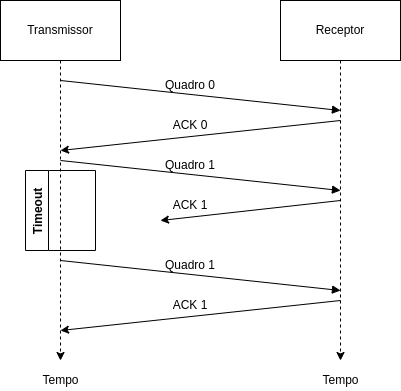
\includegraphics[width=.8\textwidth]{stop_and_wait}
    \caption{\label{fig:stop_and_wait}Fluxo de execução no tempo do algoritmo stop and wait}
\end{figure}

\section{Proposta de Arquitetura}\label{Proposta de Arquitetura}

Após decidir os algoritmos e dispositivos mais adequados para implementação foi idealizada a arquitetura do projeto.

\cleardoublepage
\begin{figure}[!htb]
    \centering
    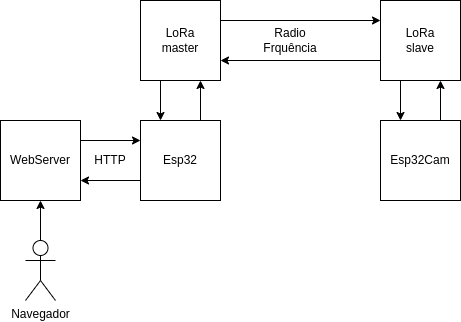
\includegraphics[width=.9\textwidth]{arch}
    \caption{\label{fig:arch}Proposta de arquitetura para implementação}
\end{figure}

O foco principal da arquitetura é implementar uma rede LoRa estrela a qual possui um ``mestre'', chip com id 0, e diversos \textit{slaves}, chips com id maior que 0. O chip \textit{master} está conectado a um esp32 executando o algoritmo de receptor que será explicado na seção \nameref{Implementação}

Para teste foi criado 2 versões do código de dispositivos emissores, sendo eles:
\begin{enumerate}
    \item Sempre envia, quando recebe o ack do último frame tira uma nova foto e envia a mesma.
    \item Envia apenas quando solicitado, fica esperando até receber uma mensagem do \textit{master} dizendo para tirar uma nova foto e enviar.
\end{enumerate}

Para testar o recebimento e visualizar de maneira mais simples foi criado um acess point WiFi na qual um usuário final pode se conectar, também é disponibilizado os seguintes endpoints no web server:

\begin{itemize}
    \item\textbf{/lora\_img}
        \begin{itemize}
            \item Objetivo: Mostrar no dispositivo do usuário uma imagem JPEG com a última foto salva no dispositivo;
            \item Método: GET;
            \item Retorna: image/jpeg
        \end{itemize}
    \item\textbf{/req\_img/\{\}}
        \begin{itemize}
            \item Objetivo: Fazer com que o LoRa mestre envie uma mensagem pedindo ao dispositivo que tire uma foto e envie;
            \item Parâmetros na url: o id do chip LoRa que vai enviar a imagem;
            \item Método: GET;
            \item Retorna: text/plain, indicando se foi possível ou não fazer a requisição.
        \end{itemize}
\end{itemize}

\section{Implementação}\label{Implementação}

Visto a proposta de arquitetura supracitada, faz-se necessário implementar dois projetos sendo eles: um transmissor que envia uma imagem separada em diversos quadros utilizando o algoritmo stop and wait, e um receptor que recebe e serve essas imagens para outras aplicações.

\subsection{Sender}\label{Sender}
Do lado do \textit{Sender}, dispositivo que captura e envia imagens, em um primeiro momento são inicializadas a câmera e a antena LoRa. Em seguida é feita a captura de uma imagem que passa a ser dividida em partes atendendo ao tamanho máximo que pode ter o payload da mensagem que pode ser enviada pela antena LoRa. Assim, uma vez dividida a imagem inicia o seu processo de envio, no qual se envia o quadro e espera uma resposta. Caso não receba nada em determinado tempo ou receba algo que não seja o ``ACK'' esperado a mensagem será reenviada. Sendo assim em alto nível o algoritmo de envio:

\begin{lstlisting}[title=Algoritmo Stop and Wait - Sender]
void sender() {
	InitCamera();
	InitLoRa();
	TakePicture(image); // tira uma foto
	SplitImage(image); // separa image em pacotes
	while(image.sendedParts < image.totalParts) {
		SendImagePart(image.part()); // envia quadro contendo parte da imagem
		ReceivePacketCommand	(buffer); // espera ate receber um quadro
		if(buffer.messageType == ACK) {
			image.sendedParts++; // incrementa contador de imagens enviadas
		}
	}
}
\end{lstlisting}

Dessa forma o fluxo de execução do dispositivo que envia a imagem:

\cleardoublepage
\begin{figure}[h]
  \centering
  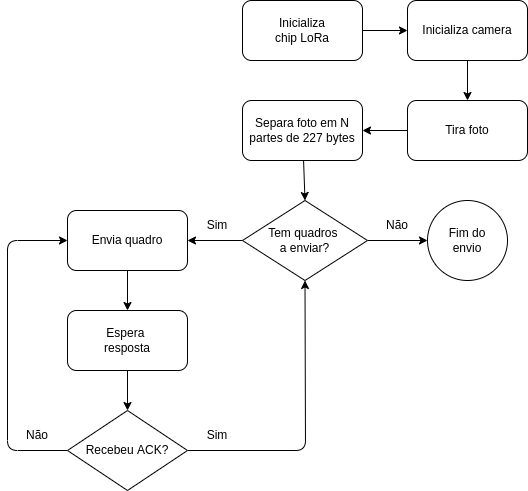
\includegraphics[width=.7\textwidth]{fluxogram_sender}
  \caption{\label{fig:sender}Fluxograma geral do algoritmo do sender.}
\end{figure}

\subsection{Receiver}\label{Receiver}
Por outro lado no \textit{receiver}, em um primeiro momento também são inicializadas as estruturas de controle, bem como é alocado um espaço que serve de buffer para colocar as partes da imagem que está sendo recebida. Após isso, o dispositivo fica esperando o recebimento de pacotes.

\begin{lstlisting}[title=Algoritmo Stop and Wait - Receiver]
void receiver() {
	InitImage(image); // inicializa estrutura de dados das imagens
	InitLoRa();
	while(true) {
		ReceivePacketCommand	(buffer); // espera ate receber um quadro
		SaveImageBytes(buffer); // salvar bytes na estrutura da imagem
		PrepareFrameCommand(); // prepara ACK
		SendPacket(); // envia ACK
		if(image.isComplete()) {
			SaveImage(image); // salvar imagem em arquivo
		}
	}
}
\end{lstlisting}
\cleardoublepage

\begin{figure}[ht]
  \centering
  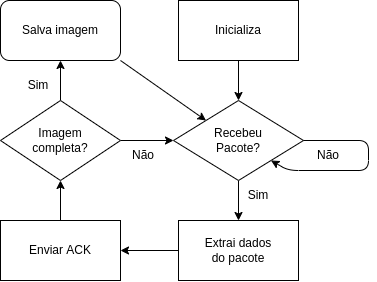
\includegraphics[width=.7\textwidth]{fluxogram_recivier}
  \caption{\label{fig:recivier}Fluxograma geral do algoritmo do receiver.}
\end{figure}

\subsection{Formato das mensagens}\label{Formato das mensagens}
Para enviar mensagens utilizando o chip LoRa, é preciso seguir o formato:
\begin{table}[h]
\caption{Estrutura padrão de mensagens LoRa.}
\centering
\begin{tabular}{llll}
\hline
\multicolumn{1}{|c|}{ID}      & \multicolumn{1}{c|}{Command} & \multicolumn{1}{c|}{Payload}       & \multicolumn{1}{c|}{CRC}     \\ \hline
\multicolumn{1}{|c|}{2 bytes} & \multicolumn{1}{c|}{1 byte}  & \multicolumn{1}{c|}{1--231 bytes} & \multicolumn{1}{c|}{2 bytes} \\ \hline
 &  &  &  \\
 &  &  &  \\
 &  &  & 
\end{tabular}
\end{table}

Sendo assim sempre os primeiros 2 bytes de uma mensagem são o id do chip que está enviando, o terceiro byte é o comando, podendo ser para realizar alguma configuração no chip, ler algum dado específico, ou simplesmente para enviar para antena $(40_{10}, 28_{16})$, seguidos de 1 a 231 bytes de mensagem e por fim os últimos 2 bytes são o CRC calculado para a mensagem específica.

Tendo uma quantidade máxima de 231 bytes para escrever os dados da imagem, optou-se pelos seguintes campos de cabeçalho:

\begin{table}[h]
\caption{Estrutura definida para o payload da mensagem.}
\centering
\begin{tabular}{cllll}
\hline
\multicolumn{5}{|c|}{Payload}    \\ \hline
\multicolumn{1}{|c|}{Type}   & \multicolumn{1}{c|}{ID}     & \multicolumn{1}{c|}{Part}   & \multicolumn{1}{c|}{Total}  & \multicolumn{1}{c|}{Message}      \\ \hline
\multicolumn{1}{|c|}{1 byte} & \multicolumn{1}{c|}{1 byte} & \multicolumn{1}{c|}{1 byte} & \multicolumn{1}{c|}{1 byte} & \multicolumn{1}{c|}{1--227 bytes} \\ \hline
\multicolumn{1}{l}{} &  &  &  &  \\
\multicolumn{1}{l}{} &  &  &  & 
\end{tabular}
\end{table}

\cleardoublepage
Sendo que:
\begin{itemize}
    \item\textbf{Type}: campo que indica como os próximos bytes devem ser interpretados, podendo ser um ACK, ou uma parte de imagem.
    \item\textbf{ID}: identificador único da imagem;
    \item\textbf{Part}: qual a parte da imagem que está nessa mensagem;
    \item\textbf{Total}: a quantidade total de partes da imagem;
    \item\textbf{Message}: os bytes da imagem
\end{itemize}

Porém caso o 1 byte, \textit{Type}, seja um ``ACK'' não terá outros campos de cabeçalho apenas um outro byte dizendo qual parte de imagem está atrelado o ``ACK''.

Dessa forma foi implementado a seguinte estrutura de dados para enviar as imagens:

\begin{lstlisting}[title=Definição da estrutura do payload]
struct _payload {
    uint8_t byte_array[APPLICATION_MAX_PAYLOAD_SIZE];
    uint8_t size;
};

struct _fields {
    uint8_t type;
    uint8_t id;
    uint8_t part;
    uint8_t last_part;
};

union ImagePart {
    _fields fields;
    _payload payload;
};
\end{lstlisting}

\section{Resultados}\label{Resultados}

A fim de avaliar o funcionamento da implementação foram realizados diversos testes, dando especial atenção para a forma como a resolução e a taxa de compressão da imagem influenciam no tamanho da mensagem enviada no payload. Os principais resultados são mostrados a continuação.

No primeiro grupo de testes realizado o foco foi avaliar como a resolução da imagem influencia no tamanho em bytes da mensagem enviada. Para isso seguiu-se os seguintes critérios:
\cleardoublepage
\begin{itemize}
    \setlength\itemsep{0.01cm}
    \item 3 fotos por resolução escolhendo sempre a mediana.
    \item Fotos tiradas do mesmo local na mesma posição;
    \item Taxa de compressão do JPEG em 0;
    \item Imagens em escala de cinza;
\end{itemize}

\begin{table}[!h]
\centering
\begin{tabular}{@{}c|c@{}}
\toprule
Resolução (pixels) & Tamanho (bytes) \\ \midrule
640$\times$480            & 73260           \\
480$\times$320            & 39139           \\
400$\times$296            & 35916           \\
320$\times$240            & 23510           \\
240$\times$176            & 14242           \\
176$\times$144            & 9147            \\ \bottomrule
\end{tabular}
\caption{Mudança de resolução afetando o tamanho da imagem}
\label{tab:resolution}
\end{table}

No segundo grupo de testes o foco foi avaliar a taxa de compressão do JPEG, sendo assim seguiu-se os critérios supracitados porém mantendo a resolução fixa em 480x320 e alterando a perda de qualidade da imagem.

\begin{table}[!h]
\centering
\begin{tabular}{@{}c|c@{}}
\toprule
Qualidade (0--63) & Tamanho (bytes) \\ \midrule
0                & 39139           \\
10               & 8456            \\
20               & 6371            \\
30               & 5613            \\
40               & 5161            \\
50               & 4842            \\
60               & 4665            \\
63               & 4616            \\ \bottomrule
\end{tabular}
\caption{Mudança de qualidade da imagem afetando o tamanho}
\label{tab:quality}
\end{table}

Avaliando também a taxa de transmissão percebeu-se que utilizando o algoritmo \textit{stop and wait} cada troca de quadros demora aproximadamente 2 segundos sendo assim pode-se calcular o tempo médio de envio de cada imagem dependendo unicamente da quantidade de quadros que a mesma ocupa.

\section{Conclusão}\label{Conclusão}
Apesar de todas as limitações da tecnologia LoRa tais como velocidade de transmissão, direção do canal, ainda é possível transmitir pequenas e comprimidas imagens com alta latência.

Sendo assim possível implementar uma rede estrela para transmissão de conteúdos maiores que o suportado por uma única mensagem LoRa (231 bytes), abrindo possibilidades para envio de imagens, arquivos e grandes mensagens.

% ----------------------------------------------------------
% ELEMENTOS PÓS-TEXTUAIS
% ----------------------------------------------------------

\postextual

% ----------------------------------------------------------
% Referências bibliográficas
% ----------------------------------------------------------
\bibliography{ref}

\end{document}
